
%(BEGIN_QUESTION)
% Copyright 2006, Tony R. Kuphaldt, released under the Creative Commons Attribution License (v 1.0)
% This means you may do almost anything with this work of mine, so long as you give me proper credit

Examine this closed-loop trend from a temperature-control process:

$$\includegraphics[width=15.5cm]{i00291x01.eps}$$

Identify whether you think this is a {\it P-only}, {\it I-only}, {\it P+I}, {\it P+D}, or full {\it PID} controller, based on the trends shown here.

\vskip 10pt

Also, identify whether this is a {\it direct-acting} or a {\it reverse-acting} controller.

\vskip 10pt

Finally, identify the problem this loop has, explaining how you can tell from the trends.

\vskip 50pt

\underbar{file i00291}
%(END_QUESTION)





%(BEGIN_ANSWER)

{\bf 2 points:} This is a {\bf P-only} controller (no integral or derivative action).  

\vskip 10pt

{\bf 2 points:} The controller is configured for {\bf reverse} action.

\vskip 10pt

{\bf 2 points:} The problem is a lack of integral action in the controller, resulting in proportional-only offset.

\vskip 10pt

{\bf 4 points:} We can identify this problem the persistent error between PV and SP.

%(END_ANSWER)





%(BEGIN_NOTES)

{\bf This question is intended for exams only and not worksheets!}.

%(END_NOTES)


